\documentclass{article}
\usepackage{iclr2027_conference,times}
\usepackage{amsmath,amssymb}
\usepackage{booktabs}
\usepackage{graphicx}
\usepackage{hyperref}
\usepackage{url}
\usepackage{microtype}
\hypersetup{hidelinks}

\title{Transient Low-Order Cues Bootstrap Compositional\\
Representations Across Transformer Scales}
\author{Anonymous Authors}

% Keep \iclrfinalcopy commented for anonymous submission.

\begin{document}
\maketitle


\begin{abstract}
We study whether training-distribution geometry can alter formation of a
higher-order predictive representation while the target conditional,
irreducible noise, marginals, and total predictable information remain fixed.
In a finite-field parent-exposed task, two uniform parents determine a modular
center and a fixed additive-noise channel determines the target. An
exploratory study found that transient full-support low-order cues advanced
predictive-state formation. We prospectively froze the architecture,
optimizer configuration, objective, evaluation protocol, onset definition,
and statistical test before confirmatory training. The confirmatory study used
held-out rules, cue permutations, and initializations with three cue doses.
Verified onset occurred in 1/8,
6/8, and 8/8 blocks. The
one-sided exact blocked Page-style test enumerated
1,679,616 assignments and gave
$p=9.5259869e-06$. All 13 nonzero-cue cells
positive at cue removal retained the representation threshold at 6M and 10M.
In a preregistered post-confirmatory robustness extension at approximately
1M and 5M core parameters, R2 advanced verified onset in all eight paired
blocks. At 1M, onset occurred in 0/4 R0 versus 4/4 R2 cells; at 5M, it occurred
in 3/4 versus 4/4. These scale results are descriptive, are excluded from the
original v3.6 $p$-value, and are not a scaling-law fit.
Temporary cue-bearing distributions therefore causally changed onset timing or
probability within the task and model family under the fixed confirmatory
protocol. The experiment does not
identify singleton mutual information alone as causal and does not establish a
universal Transformer property. In plain terms, a temporary statistical
scaffold helped the model discover a rule representation that remained useful
after the scaffold was removed.
\end{abstract}

\section{Introduction}
The central question is: \emph{How does training-distribution geometry affect
the accessibility of task-sufficient representations when the final task
information is fixed?} A representation may be statistically available yet
difficult to discover because useful optimization directions are weak, cancel
across examples, or become accessible only after other features organize. We
therefore intervene on early training-distribution geometry while holding the
target conditional and information budget fixed.

Project Kepler uses a finite-field mechanism assay motivated by, but distinct
from, its recurrent production task. The parent-exposed design intentionally
separates (1) identifying relevant variables, which the interface controls by
presenting both parents directly, from (2) composing discovered variables into
a predictive representation, which remains the learning problem. The present
paper does not claim that the recurrent task has been solved.

Version 3.5 is exploratory discovery. Before confirmatory training, all
outcome definitions and analysis choices were prospectively frozen. Version
3.6 is a prospectively frozen confirmatory replication using held-out rules,
cue permutations, and initializations; discovery data are excluded from its
primary $p$-value. After that test was complete, we separately preregistered a
minimal 1M/5M robustness extension. It reuses the frozen outcomes but does not
enter the v3.6 inference. The aim is neither a scaling law nor a universal
intelligence principle; it is a bounded causal test plus a post-confirmatory
scale check within one task and model family. Figure~\ref{fig:task} summarizes
the construction and cue schedule.

\begin{figure}[tb]
\centering
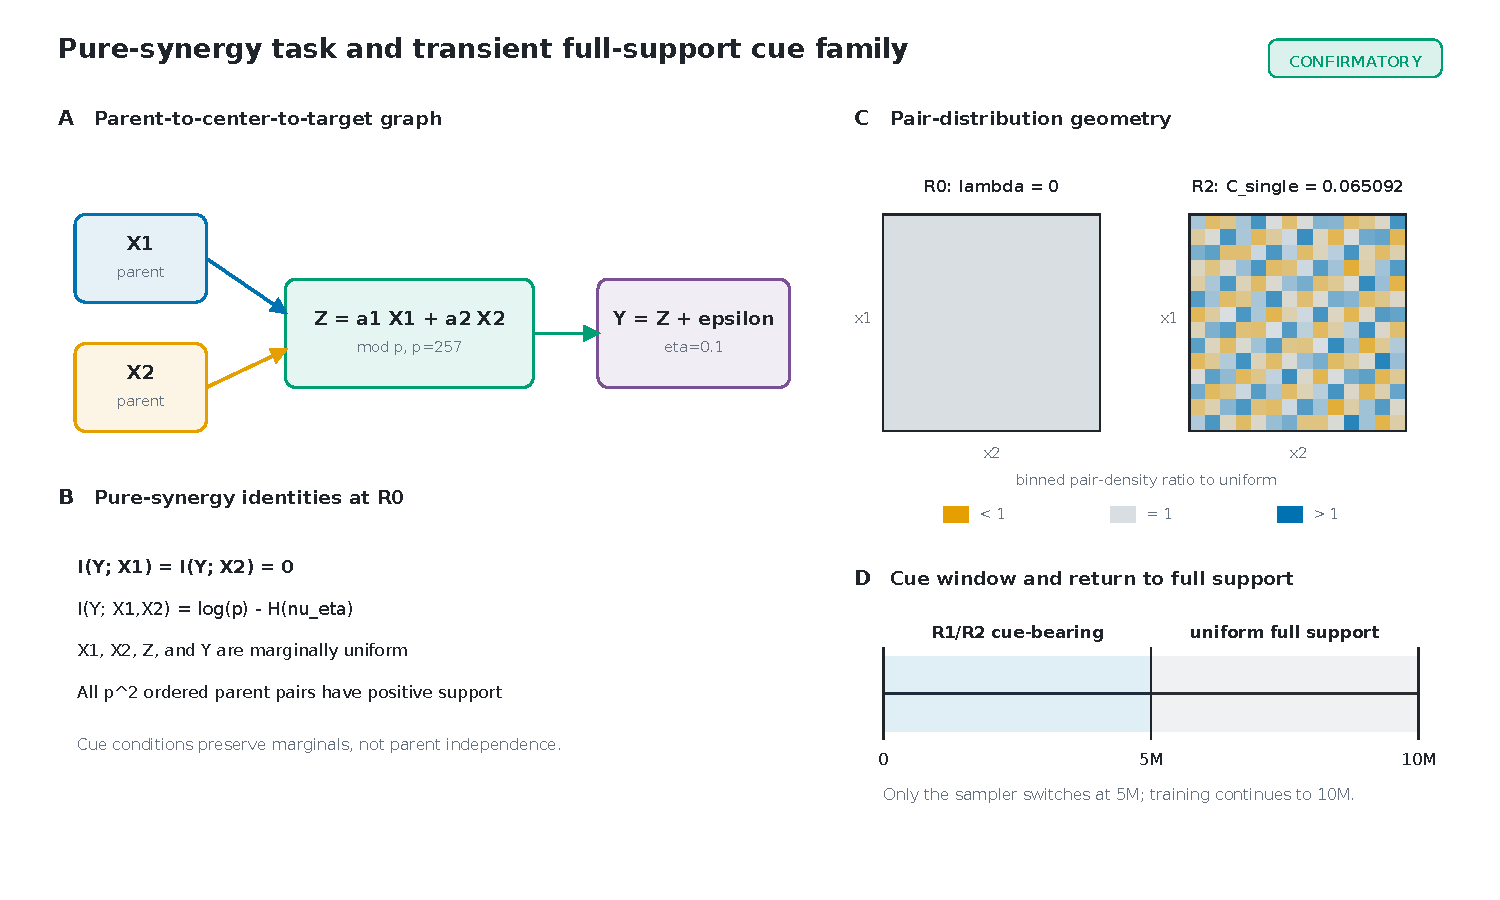
\includegraphics[width=\linewidth]{figures/fig01_task_cue_schematic.pdf}
\caption{Controlled task, pure-synergy identities, R0-versus-R2
pair-distribution geometry, and transient cue schedule. Binned pair-density
ratios and all displayed values are generated from frozen distribution JSON.}
\label{fig:task}
\end{figure}

\section{Related Work}
\paragraph{Grokking and delayed generalization.}
Modular-arithmetic grokking studies established that small neural networks can
generalize long after achieving near-perfect training performance under a
fixed training distribution \cite{power2022grokking}. Follow-up work
connected delayed generalization to structured representation learning and its
training dynamics \cite{liu2022understanding}. This paper does not offer a
universal explanation of grokking. It instead asks whether the geometry of the
\emph{early} training distribution, with the final conditional and
information budget held fixed, changes the accessibility or timing of a
delayed representational transition.

\paragraph{Mechanistic interpretability of modular arithmetic.}
Mechanistic analyses of modular addition have recovered Fourier-like internal
representations and circuits implementing trigonometric structure
\cite{nanda2023progress}, while other architectures and initializations can
learn qualitatively different modular-addition algorithms
\cite{zhong2023clock}. Here, fixed-Fourier probes are diagnostics alongside
linear and fixed-capacity MLP probes. Probe accuracy establishes extractability
under the specified probe, not causal use by the model
\cite{hewitt2019probes,belinkov2022probes}. We do not assume that a specific
Fourier circuit must be learned, and the causal result concerns the timing or
probability of task-sufficient representation formation rather than
identification of a unique circuit.

\paragraph{Curriculum learning.}
Classic curricula order examples by difficulty
\cite{bengio2009curriculum,hacohen2019curriculum}; self-paced methods adapt
selection to the learner \cite{jiang2015selfpaced}; and continuation methods
smooth or deform an optimization problem \cite{mobahi2016diffusion}. The
present intervention is a \emph{distributional curriculum} whose distinctive
control is preservation of the target conditional, Bayes entropy, total
predictable information, and full pair support. It changes the geometry of a
full-support sampling distribution during an early window. We call this
narrower intervention \emph{distributional bootstrapping of representation
formation}.

\paragraph{Optimization path dependence.}
Learning dynamics can show long plateaus, rapid transitions, and strong
dependence on initialization even in analytically tractable deep linear
networks \cite{saxe2014exact}. This motivates studying training paths, but it
does not by itself identify the mechanism in the present Transformer. Our
gradient statistics are therefore treated as descriptive correlates rather
than causal mediators.

\paragraph{Partial Information Decomposition.}
Partial Information Decomposition separates redundant, unique, and
synergistic contributions in multivariate information
\cite{williams2010pid}. Multiple operationally motivated decompositions
exist \cite{bertschinger2014unique}, so synergy language depends on the
adopted definition. The full-support base task is a pure-synergy construction
only in the limited operational sense needed here: singleton predictive
information is zero while joint predictive information is nonzero. We do not
attempt a full PID decomposition of the cue distributions or learned
representations.

\section{Controlled finite-field task}
The field size is $p=257$. The predictive center is
$z=a_1x_1+a_2x_2 \bmod p$, and $y=z+\epsilon \bmod p$ with
$P(\epsilon=0)=1-\eta$, $P(\epsilon=r)=\eta/(p-1)$ for $r\ne0$, and
$\eta=0.1$. Thus $H(Y\mid X_1,X_2)=0.879601$ nats, and the
target conditional is unchanged across conditions. The primary metric is
\[
R=\frac{\mathbb{E}_h D_{\rm KL}(q_h\Vert p_\theta)}
{\log p-H(\nu_\eta)}.
\]
A uniform predictor has $R=1$ and the oracle has $R=0$. Objective,
evaluation, bootstrap, and probe details appear in Supplementary Methods.

\section{Pure-synergy information structure}
Under uniform full support, $X_1,X_2,Z,Y$ are uniform,
$I(Y;X_1)=I(Y;X_2)=0$, and
$I(Y;X_1,X_2)=4.66948$ nats. The scalar cue index orders
selected constructed distributions; it is not a unique-information percentage.

\section{Full-support cue-family construction}
For $z=a_1x_1+a_2x_2 \bmod p$, the prospectively frozen cue family was
\[
P_{\lambda,m}(x_1,x_2)
=\frac{1-\lambda}{p^2}
+\frac{\lambda}{mp}
\mathbf{1}\!\left[(z-cx_1)\bmod p\in B_m\right],
\]
where $B_m$ is a frozen size-$m$ subset induced by the cue permutation and
$c$ is its frozen cue coefficient. Cue dose was summarized by
\[
C_{\mathrm{single}}
=\frac{I(Y;X_1)+I(Y;X_2)}{I(Y;X_1,X_2)}.
\]
At $\lambda=0$, the distribution is uniform full support. For every
registered nonzero dose, all pair probabilities remain positive and both
parent marginals remain uniform, although $X_1$ and $X_2$ need not remain
jointly independent. $Z$ and $Y$ remain uniform; the target conditional,
Bayes entropy, and joint predictable information remain fixed.
$C_{\mathrm{single}}$ is an operational cue index, not a PID
unique-information fraction, and it does not isolate singleton mutual
information from other distributional geometry. Figure~\ref{fig:task}
compares R0 with one cue-bearing distribution.
Table~\ref{tab:table01-distribution-invariants-main} gives a representative
R0/R1/R2 summary. The complete registered audit is included as
machine-readable supplementary material, together with the derivation and
deterministic root-solving protocol.

\begin{table}[!htbp]
\centering
\caption{Representative confirmatory R0/R1/R2 distributions. H cond. is H(Y|X1,X2); complete registered audits appear in the Supplement.}
\label{tab:table01-distribution-invariants-main}
\small
\setlength{\tabcolsep}{4pt}
\begin{tabular}{lrrrrrr}
\toprule
Condition & C single & Min pair P & Max marg. err. & H cond. (nats) & Joint-I err. & Full support \\
\midrule
R0 & 7.608e-16 & 1.514e-05 & 9.107e-18 & 0.879601 & 1.066e-14 & yes \\
R1 & 0.016 & 1.237e-05 & 1.735e-18 & 0.879601 & 0 & yes \\
R2 & 0.065092 & 9.379e-06 & 1.301e-18 & 0.879601 & 0 & yes \\
\bottomrule
\end{tabular}
\end{table}


\section{Exploratory discovery experiment}
Version 3.5 used rule $(45,36)$, five paired seeds, four ordered $m=64$ doses,
and two matched-index geometry controls. Verified onset occurred in
0/5 C0, 5/5 C1, 5/5 C2, and
5/5 C3 seeds. The exploratory exact test gave
$p=1.6075103e-05$. These observations selected frozen
confirmatory conditions and definitions; they are not confirmatory data.

\begin{figure}[tb]
\centering
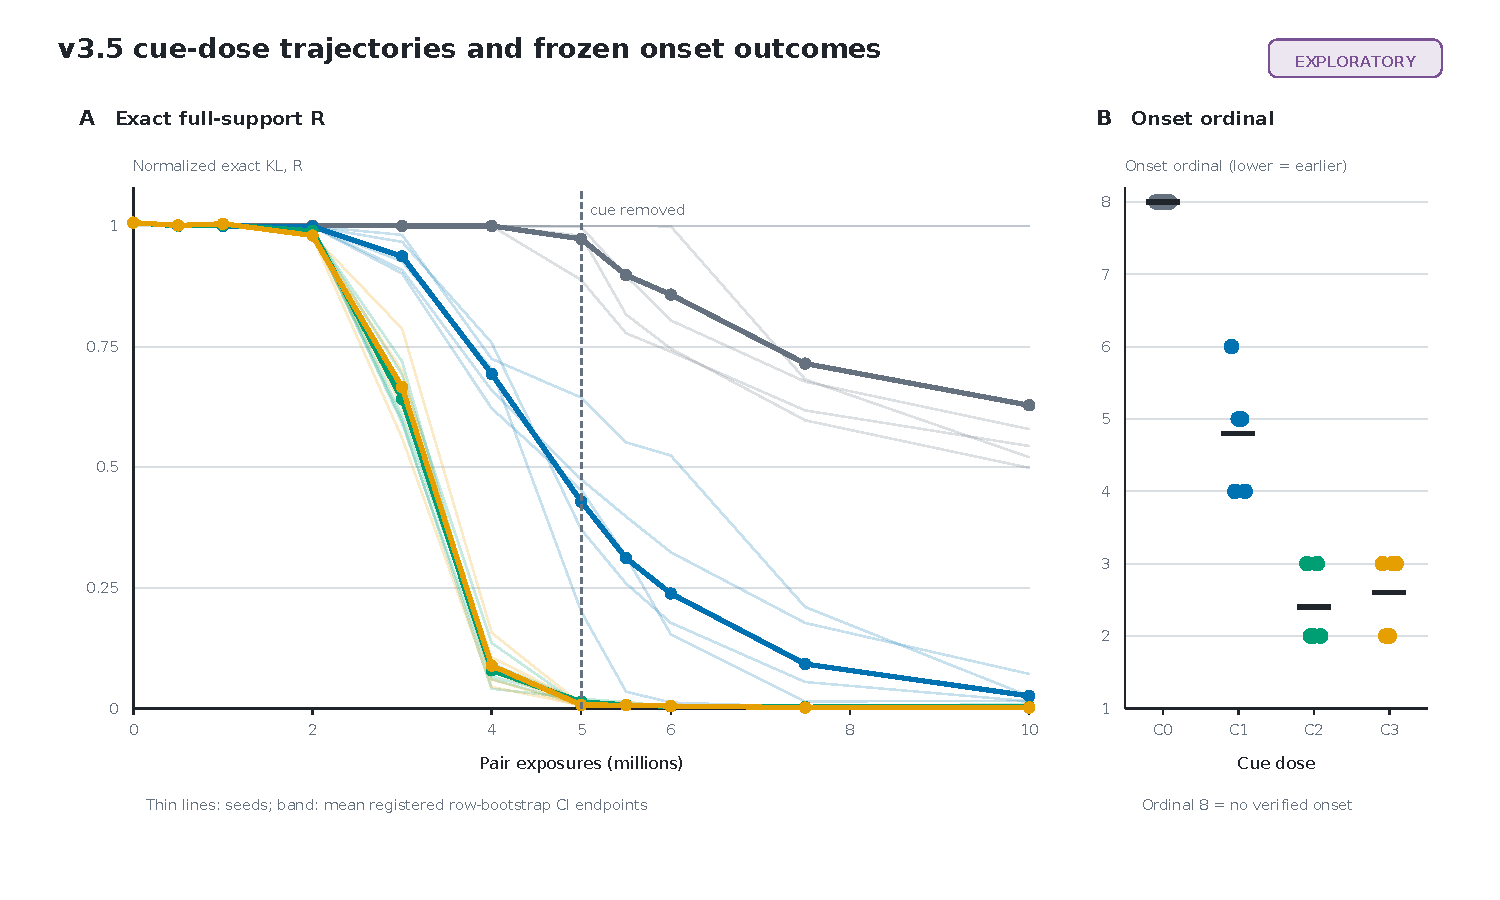
\includegraphics[width=\linewidth]{figures/fig02_v35_dose_trajectories.pdf}
\caption{Exploratory v3.5 R trajectories and onset outcomes. Bands are means
of registered row-bootstrap endpoints, not new group-level intervals.}
\label{fig:v35-trajectories}
\end{figure}

\begin{table}[!htbp]
\centering
\caption{Exploratory onset and establishment summary; complete checkpoint coding appears in the Supplement.}
\label{tab:table02-v35-exploratory-outcomes-main}
\small
\setlength{\tabcolsep}{4pt}
\begin{tabular}{lrrrrr}
\toprule
Condition & Onset by 5M & Onset by 10M & Established by 10M & Mean R, 5M & Mean R, 10M \\
\midrule
C0 & 0 & 0 & 0 & 0.973341 & 0.628411 \\
C1 & 2 & 5 & 5 & 0.428643 & 0.025721 \\
C2 & 5 & 5 & 5 & 0.013564 & 0.003252 \\
C3 & 5 & 5 & 5 & 0.007108 & 0.00162 \\
\bottomrule
\end{tabular}
\end{table}

Figure~\ref{fig:v35-trajectories} and
Table~\ref{tab:table02-v35-exploratory-outcomes-main} report the discovery
trajectories and compact frozen outcomes. Complete coding is included in the
machine-readable supplement.

\section{Prospectively frozen confirmatory replication}
Version 3.6 was a prospectively frozen confirmatory replication using held-out
rules, cue permutations, and initializations. Crossing two held-out rules, two
held-out cue permutations, and two held-out initialization seeds yielded eight
paired blocks and 24 trajectories. R0, R1, and R2 shared initial weights and
all non-condition random fields within each block. The primary inference unit
was the eight rule $\times$ permutation $\times$ initialization blocks. The 24
trajectories were paired condition observations---three per block---not 24
independent inferential units. Verified onset occurred in
1/8,
6/8, and 8/8 blocks. The observed
Page-style statistic was 110.0. Under the
prospectively frozen sharp null, condition labels were exchangeable within
each block. Exactly
16 of 1,679,616
assignments were at least as large; the exact upper-tail count included the
observed assignment. This gave one-sided
$p=9.5259869e-06$.

\begin{figure}[tb]
\centering
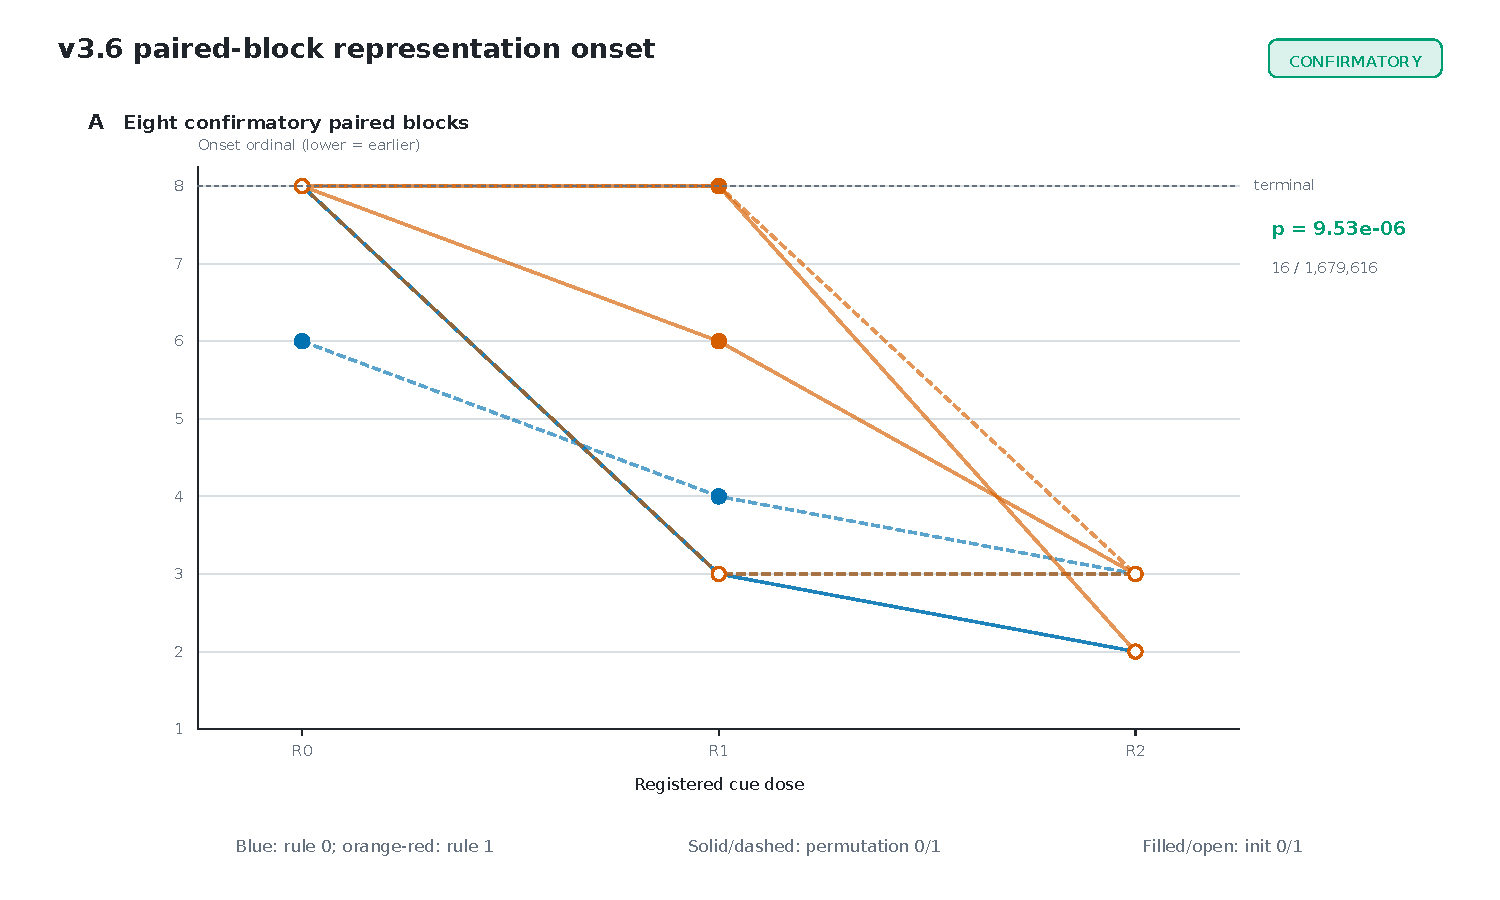
\includegraphics[width=\linewidth]{figures/fig03_v36_paired_onset.pdf}
\caption{Paired terminal-coded onset ordinals for all eight confirmatory
blocks.}
\label{fig:v36-onset}
\end{figure}

\begin{figure}[tb]
\centering
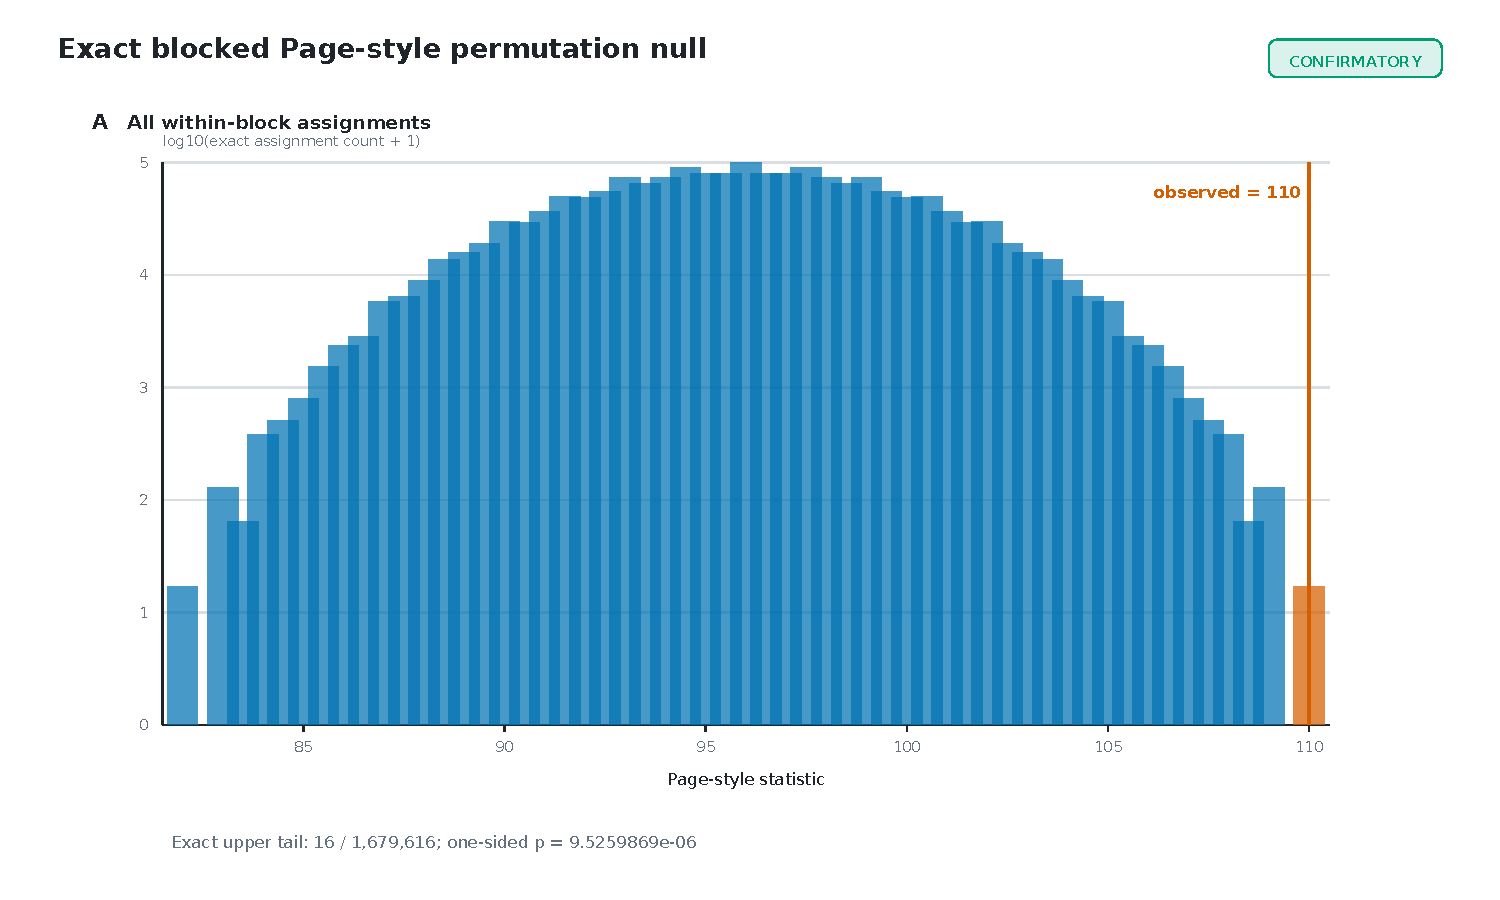
\includegraphics[width=\linewidth]{figures/fig04_v36_exact_null.pdf}
\caption{Exact v3.6 permutation null. Version 3.5 is excluded.}
\label{fig:exact-null}
\end{figure}

\begin{table}[!htbp]
\centering
\caption{Confirmatory outcomes across eight paired inference blocks; complete coding appears in the Supplement.}
\label{tab:table03-v36-confirmatory-outcomes-main}
\small
\setlength{\tabcolsep}{4pt}
\begin{tabular}{lrrrrr}
\toprule
Condition & Onset by 5M & Onset by 10M & Established by 10M & Mean R, 5M & Mean R, 10M \\
\midrule
R0 & 0 & 1 & 2 & 1.000239 & 0.432743 \\
R1 & 5 & 6 & 6 & 0.303076 & 0.110766 \\
R2 & 8 & 8 & 8 & 0.04371 & 0.005181 \\
\bottomrule
\end{tabular}
\end{table}

\begin{table}[!htbp]
\centering
\caption{Primary confirmatory exact test. Stratified tests are secondary, nominal, and not multiplicity-adjusted; full results appear in the Supplement.}
\label{tab:table04-exact-tests-main}
\small
\setlength{\tabcolsep}{4pt}
\begin{tabular}{lrrrrr}
\toprule
Analysis & Blocks & Assignments & Statistic & Upper tail & One-sided p \\
\midrule
primary & 8 & 1679616 & 110 & 16 & 9.526e-06 \\
\bottomrule
\end{tabular}
\end{table}

\begin{table}[!htbp]
\centering
\caption{Mean paired differences, higher registered dose minus lower registered dose; medians and audit fields appear in the Supplement.}
\label{tab:table05-paired-R-differences-main}
\small
\setlength{\tabcolsep}{4pt}
\begin{tabular}{lrrrr}
\toprule
Comparison & Blocks & Mean delta R, 5M & Mean delta R, 10M & Mean onset delta \\
\midrule
R1\_minus\_R0 & 8 & -0.697162 & -0.321977 & -3 \\
R2\_minus\_R0 & 8 & -0.956528 & -0.427562 & -5.125 \\
R2\_minus\_R1 & 8 & -0.259366 & -0.105585 & -2.125 \\
\bottomrule
\end{tabular}
\end{table}

Figures~\ref{fig:v36-onset} and \ref{fig:exact-null} show the paired
onset ordinals and exact null.
Tables~\ref{tab:table03-v36-confirmatory-outcomes-main},
\ref{tab:table04-exact-tests-main}, and
\ref{tab:table05-paired-R-differences-main} report compact confirmatory
outcomes, the primary exact test, and mean paired differences. Complete fields
and the transition-coding audit are in the machine-readable supplement. Rule- and
permutation-stratified tests are secondary, nominal, and not multiplicity-adjusted.

\section{Representation persistence after cue removal}
At 5M only the sampler changed for nonzero-cue runs. Zero-step checks verified
unchanged outputs and model, optimizer, scheduler, exposure, and RNG state.
All 13 threshold-positive R1/R2 cells remained positive at 6M
and 10M, supporting learning-path preconditioning rather than a permanently
required shortcut.

\begin{figure}[tb]
\centering
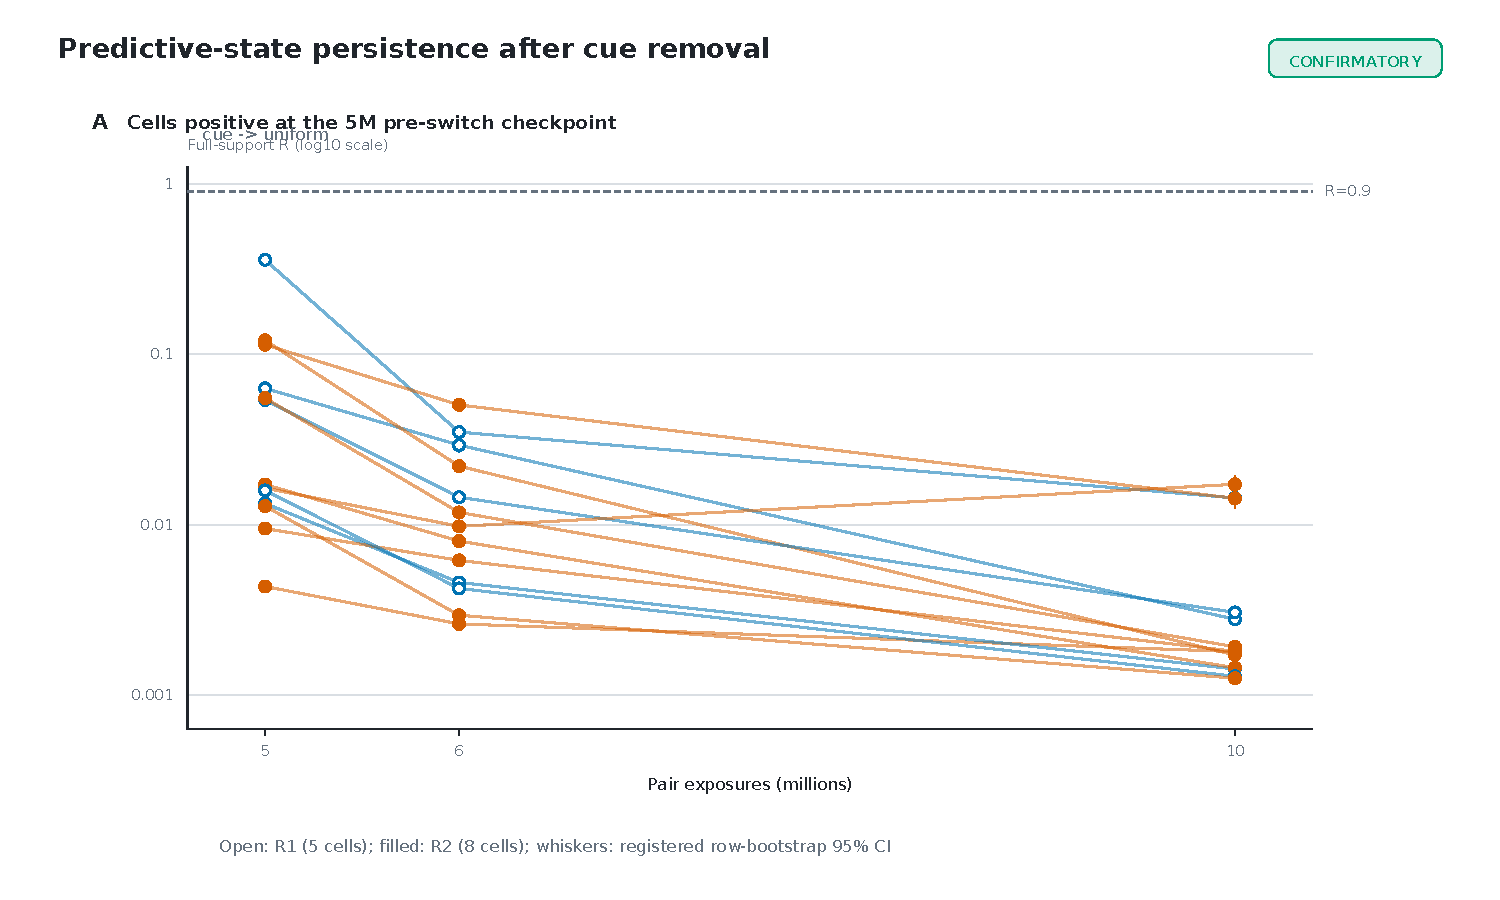
\includegraphics[width=\linewidth]{figures/fig05_v36_persistence.pdf}
\caption{Persistence after return to uniform full support. Whiskers are
registered first-parent-row bootstrap intervals.}
\label{fig:persistence}
\end{figure}

\begin{table}[!htbp]
\centering
\caption{Confirmatory retention after return to uniform full support; complete exploratory and confirmatory records appear in the Supplement.}
\label{tab:table06-cue-removal-persistence-main}
\small
\setlength{\tabcolsep}{4pt}
\begin{tabular}{lrrr}
\toprule
Condition & Positive at 5M & Retained at 6M & Retained at 10M \\
\midrule
R1 & 5 & 5 & 5 \\
R2 & 8 & 8 & 8 \\
\bottomrule
\end{tabular}
\end{table}

Figure~\ref{fig:persistence} and
Table~\ref{tab:table06-cue-removal-persistence-main} report the persistence
result. The complete exploratory and confirmatory switch audit is included in
the machine-readable supplement.

\section{Post-confirmatory cross-scale robustness}
After completing v3.6, we preregistered a minimal extension at approximately
1M and 5M core parameters. Width was the only scaled architectural quantity;
depth, heads, input interface, $p=257$, $\eta=0.1$, optimizer
parameterization, exact soft-label objective, and absolute-exposure schedule
were unchanged. Two frozen rules and two paired initialization seeds were
crossed with R0 and R2, giving four paired blocks per scale and 16 trajectories.
R0/R2 shared initialization and non-condition randomness within every block.

A preregistered engineering/learnability pilot first ran one pair per scale.
Both scales passed memory, throughput, checkpoint-resume, non-saturation, and
identifiability gates; a favorable cue effect was not required. All 16 runs
then used cue-bearing sampling through 5M and uniform full support from 5M to
10M. All zero-step switch checks and all 176 checkpoint sidecar checks passed.

R2 advanced the registered terminal-coded onset ordinal in 4/4 blocks at each
scale (Table~\ref{tab:scale-robustness-main}). At 1M, verified onset occurred
in 0/4 R0 and 4/4 R2 trajectories; at 5M it occurred in 3/4 and 4/4. All R2
trajectories retained the onset threshold at 6M and 10M after cue removal.
Every paired block and its frozen metrics appear in
Tables~\ref{tab:scale-robustness-blocks}--\ref{tab:scale-robustness-metrics}.
This extension is post-confirmatory descriptive evidence: it is excluded from
the original v3.6 $p$-value, no new combined $p$-value is computed, and two
scales do not constitute a scaling-law fit.

\begin{table}[t]
\caption{Post-confirmatory cross-scale robustness. ``Earlier'' compares the
registered terminal-coded onset ordinal within each paired block. The extension
is excluded from the v3.6 $p$-value and is not a scaling-law fit.}
\label{tab:scale-robustness-main}
\centering
\small
\begin{tabular}{lrrrrrr}
\toprule
Scale & Core params & Width & R0 onset & R2 onset & R2 earlier & Mean $\Delta$ ordinal \\
\midrule
1M & 1,046,400 & 120 & 0/4 & 4/4 & 4/4 & -5.25 \\
5M & 5,039,232 & 264 & 3/4 & 4/4 & 4/4 & -3.75 \\
\bottomrule
\end{tabular}
\end{table}


\section{Rule and cue-geometry heterogeneity}
R1 onset occurred in 4/4 rule-0 and 2/4 rule-1
blocks, while R2 onset occurred in 4/4 and 4/4.
The ordered effect spans both rules but the mid-dose response is
rule-dependent. In exploratory matched-index controls, concentrated and
diffuse geometries differed from $m=64$, so equal cue-index values are not
interchangeable.

\begin{figure}[tb]
\centering
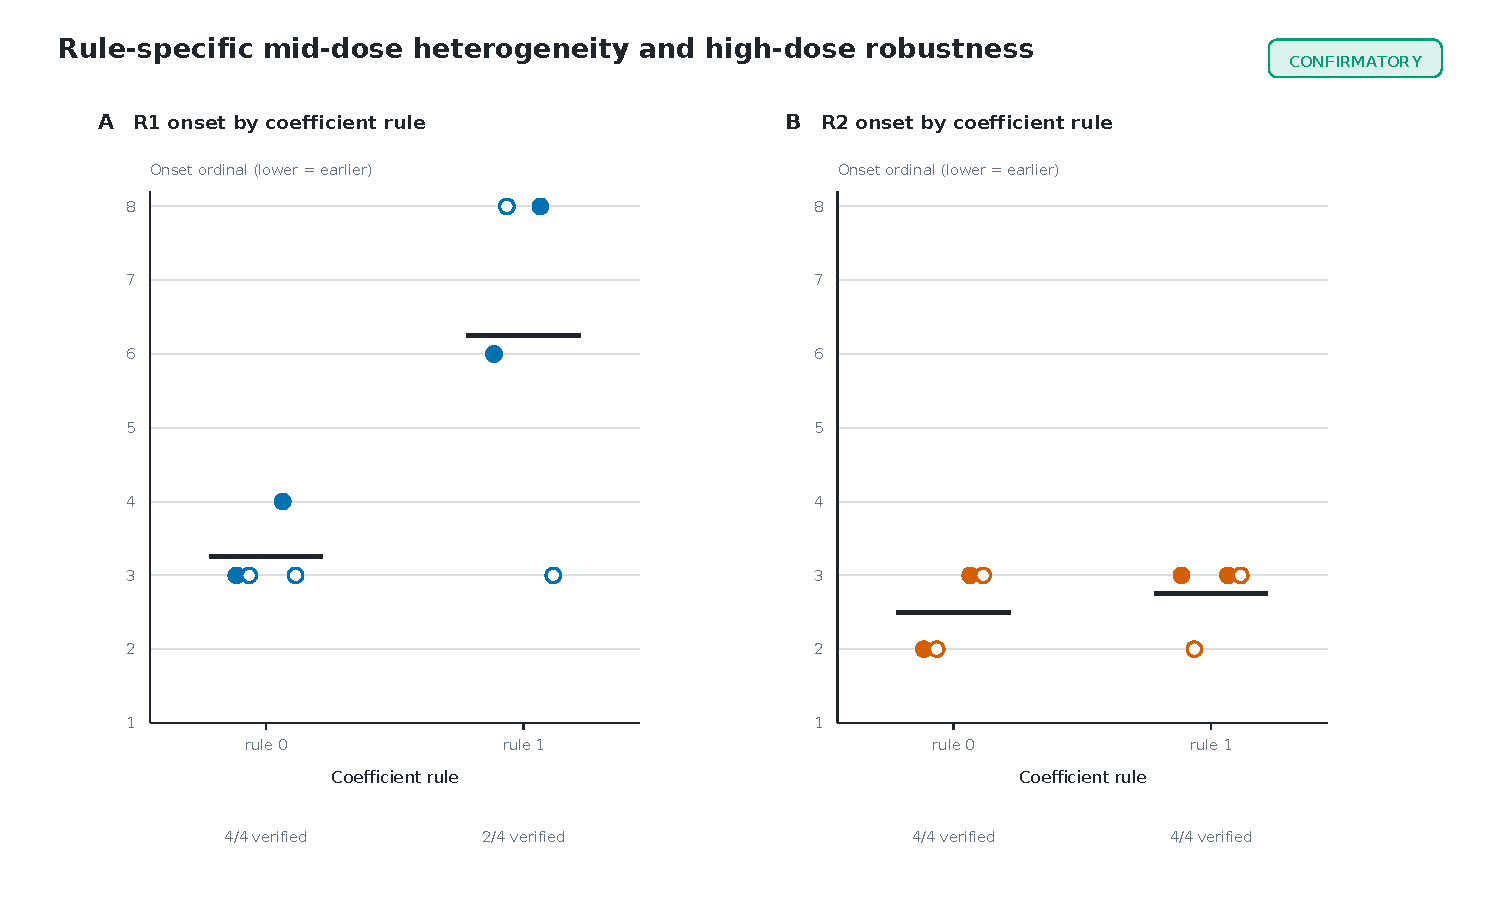
\includegraphics[width=\linewidth]{figures/fig06_v36_rule_heterogeneity.pdf}
\caption{Rule-specific R1 heterogeneity and R2 robustness.}
\label{fig:rule-heterogeneity}
\end{figure}

\begin{figure}[tb]
\centering
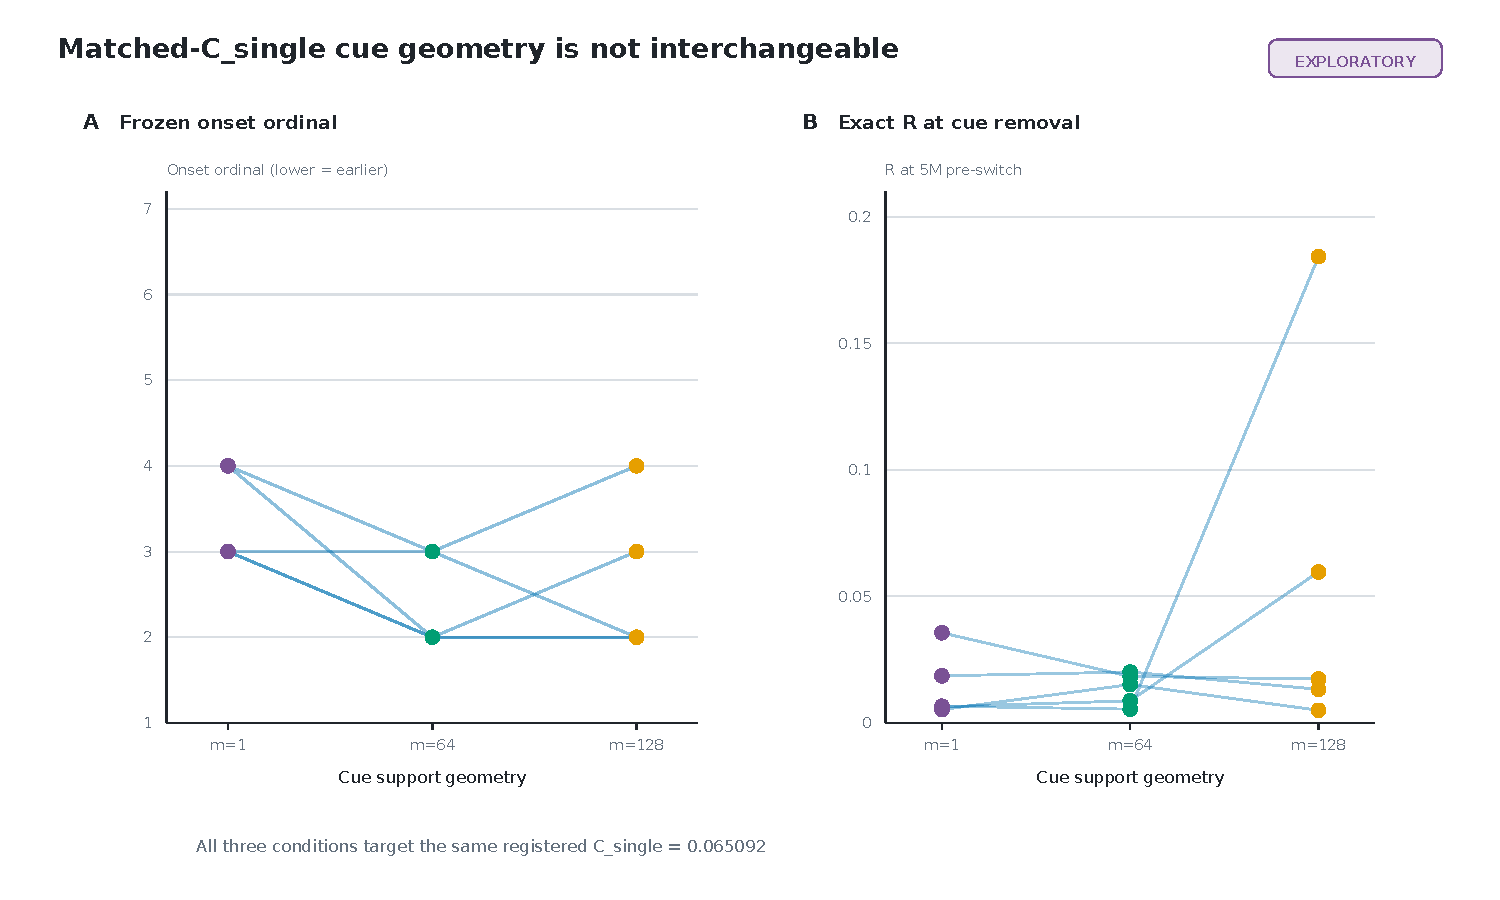
\includegraphics[width=\linewidth]{figures/fig07_v35_geometry_comparison.pdf}
\caption{Exploratory matched-index geometry comparison.}
\label{fig:geometry}
\end{figure}
Figures~\ref{fig:rule-heterogeneity} and \ref{fig:geometry} separate the
confirmatory rule comparison from the exploratory geometry comparison.

\section{Discussion}
Temporary cue-bearing full-support distributions changed whether or when the
Transformer trained under the prospectively frozen protocol formed the
modular predictive center. The target
conditional, marginals, irreducible noise, total pairwise predictable
information, architecture, optimizer, and objective were held fixed.
Persistence after cue removal indicates that the early distribution altered
the learning path rather than supplying a permanently required feature.
Heterogeneity across rules and geometries rejects an explanation based on the
scalar cue index alone. The post-confirmatory 1M/5M extension preserved the
paired direction in all eight new blocks, while the differing R0 onset rates
show that scale changes baseline learnability. This robustness result does not
extend the original confirmatory inference or justify a scaling law.

\subsection{Possible mechanism: symmetry breaking and optimization accessibility}
Pure synergy removes singleton predictive signal from the population
distribution. In the tested parameterization, this condition was associated
with weak and poorly aligned early gradients. Cue-bearing distributions
introduced lower-order statistical asymmetries that may have changed early
gradient alignment and optimization accessibility. One possible consequence
is an earlier path toward composing both parents; after the task-sufficient
representation forms, the cue is no longer required. This is an
experiment-bounded interpretation, not a theorem that gradients generally
vanish under pure synergy.

Three observations are consistent with this account: onset was ordered by
registered cue dose, threshold-positive representations persisted after cue
removal, and the frozen gradient audits showed changes in gradient coherence
around observed transitions. This is mechanistic interpretation, not a causal
mediation result. \emph{Gradient statistics are correlates of transition
dynamics, not identified causal mediators.} The data do not establish a
universal loss-landscape mechanism or a unique circuit.

\subsection{Practical implication: distributional bootstrapping}
The result suggests a possible design principle: temporary training
distributions can be used to improve access to otherwise hard-to-reach
compositional representations when the final task distribution contains
higher-order dependencies. This is a hypothesis for bounded, auditable
interventions, not a claim that all AI training should use low-order cues.

\section{Limitations}
First, model scale is sampled only at approximately 1M, 2M, and 5M core
parameters, with just four post-confirmatory pairs at each new scale; this is
not a scaling-law design. Second, the parent-exposed interface
intentionally controls variable identification; recurrent context discovery
and variable selection remain future work. Third, exact soft-label training
isolates representation formation from sampled-label variance; sampled-token
training remains future work. Fourth, finite-field modular arithmetic is a
controlled model organism rather than a proxy for the full range of
natural-data learning. Fifth, the experiments identify a distribution
intervention but do not establish a universal loss-landscape mechanism.

The study also uses one field size, one noise level, a finite checkpoint grid,
and eight confirmatory blocks. The exact test is valid for the frozen
randomization structure but does not make the tested rules a population sample
of all modular tasks. The 0--5M cue window coincided with the prospectively
frozen 5M learning-rate warmup, and cue timing was not crossed with optimizer
phase. Cue conditions preserved both parent marginals but changed their joint
distribution, so the intervention is not a marginal-frequency manipulation
alone. Dependence beyond the tested widths, field size, noise level, input
interface, and exact soft labels remains open. The result is not a universal Transformer
claim, not a thermodynamic phase transition, and not evidence that the
recurrent production task is solved. These results are excluded from the
original v3.6 $p$-value.

\subsection*{Reproducibility statement}
The confirmatory and post-confirmatory results and their frozen hashes are
recorded in the anonymous supplementary artifact package. Frozen hashes,
environment, test definitions, counts, and provenance are indexed in the
package. The lightweight verifier recomputes distribution audits, transition
coding, all 1,679,616 exact v3.6 assignments, scale summaries, figures, and
tables without optimizer steps.

\subsection*{Data and code availability}
Code, manifests, result JSON, source data, and verification scripts are
included in the repository. Checkpoints are referenced by SHA-256 sidecars and
are unnecessary for lightweight verification.

\subsection*{AI use statement}
Generative AI tools were used to discuss and refine hypotheses and experimental
methodology; implement, review, and test research software; inspect registered
results; and draft, edit, structure, and format the manuscript and artifacts.
No generative model supplied or altered experimental observations or labels;
all synthetic task data were produced by audited code. The human authors
selected and approved all
preregistrations, stopping rules, analyses, interpretations, and claims; they
verified AI-assisted code with automated tests and frozen hash audits and
reviewed the reported values against machine-readable results. The authors take
responsibility for the final content, including text, claims, code, and
artifacts produced with the aid of generative AI.

\bibliographystyle{iclr2027_conference}
\bibliography{references}

\appendix
\section{Supplementary methods}
\subsection{Task objective, evaluation, and probes}
Exact soft-label cross-entropy was used throughout the parent-exposed
experiments: at each observed pair, the target was the analytic noisy
conditional rather than one sampled label. Evaluation enumerated all
66,049 ordered parent pairs. Every checkpoint recorded exact conditional KL,
normalized $R$, center accuracy, center probability, predictive entropy, and a
2,000-replicate first-parent-row bootstrap interval. Selected checkpoints
included layer-wise linear, fixed-Fourier, and fixed-capacity MLP probes.

\subsection{Cue-family construction and audit}
Frozen cue permutations and coefficients reweighted the complete pair space
while preserving strictly positive probability for every pair. Lambda was
solved by deterministic root finding for each prospectively frozen target, not
selected from model outcomes. Exhaustive enumeration verified marginal
uniformity, conditional invariance, joint information, and full support.

\subsection{Model and optimization}
The v3.6 confirmatory manifest instantiated the architecture and optimization
settings frozen from v3.5. It records
2,045,568 core
parameters, width 168, batch size
4,096, exact soft-label cross-entropy, AdamW
learning rate $3\times10^{-4}$,
betas
$(0.9,0.95)$, weight decay
0.1, clipping at 1.0,
5M warmup exposures, and an
absolute-exposure cosine schedule.

\subsection{Transition coding}
Probe checkpoints were 2M, 3M, 4M, 5M, 6M, 7.5M, and 10M. Onset required
$R<0.9$ and layer-6 linear accuracy above 0.5, retained at the next checkpoint.
Establishment required $R<0.1$, center accuracy above 0.9, and layer-6 linear
accuracy above 0.9.

\subsection{Exact test}
Within-block terminal onset ordinals were converted to doubled midranks, with
earlier onset ranked higher. All six label assignments were combined across
eight blocks, giving $6^8=1,679,616$ assignments.
Under the sharp null, the R0/R1/R2 labels were exchangeable within each block.
The one-sided upper tail included the observed assignment.

\subsection{Post-confirmatory scale protocol and complete paired outcomes}
The separately frozen scale manifest crossed target core-parameter counts 1M
and 5M with two v3.6 coefficient rules, two v3.6 initialization seeds, and R0
versus R2. Widths 120 and 264 were selected by the unchanged width-only rule,
yielding 1,046,400 and 5,039,232 actual core parameters. Each paired block
shared initialization and every non-condition random field. The target
conditional, exact soft-label objective, optimizer protocol, 5M switch, and
registered probe grid were unchanged. The pilot gate used only engineering and
identifiability criteria. The analysis reports all blocks descriptively and
does not combine them with the v3.6 randomization test.

\begin{table}[t]
\caption{Every post-confirmatory paired block. Onset and establishment use the
unchanged v3.6 definitions. A dash denotes no verified event by 10M; persistence
reports whether the R2 onset threshold was retained at 6M and 10M after cue
removal.}
\label{tab:scale-robustness-blocks}
\centering
\small
\begin{tabular}{llrrrrll}
\toprule
Scale & Rule & Seed & R0 onset & R2 onset & $\Delta$ & R0/R2 est. & R2 persist. \\
\midrule
1M & 0 & 0 & -- & 4M & -5 & -- / 5M & yes / yes \\
1M & 0 & 1 & -- & 3M & -6 & -- / 5M & yes / yes \\
1M & 1 & 0 & -- & 4M & -5 & -- / 6M & yes / yes \\
1M & 1 & 1 & -- & 4M & -5 & -- / 7.5M & yes / yes \\
5M & 0 & 0 & -- & 3M & -6 & -- / 4M & yes / yes \\
5M & 0 & 1 & 5M & 3M & -2 & 6M / 3M & yes / yes \\
5M & 1 & 0 & 7.5M & 3M & -4 & 10M / 4M & yes / yes \\
5M & 1 & 1 & 6M & 3M & -3 & 10M / 4M & yes / yes \\
\bottomrule
\end{tabular}
\end{table}

\begin{table}[t]
\caption{Registered 10M outcomes in every post-confirmatory paired block.
Columns give exact full-support $R$, exact center accuracy, and the registered
layer-6 linear-probe accuracy for R0/R2.}
\label{tab:scale-robustness-metrics}
\centering
\small
\begin{tabular}{llrrrrrr}
\toprule
Scale & Rule/seed & $R_0$ & $R_2$ & Center$_0$ & Center$_2$ & Probe$_0$ & Probe$_2$ \\
\midrule
1M & 0/0 & .5982 & .0027 & .0492 & 1.0000 & .1333 & 1.0000 \\
1M & 0/1 & .7063 & .0038 & .0257 & 1.0000 & .0895 & 1.0000 \\
1M & 1/0 & .5785 & .0045 & .0766 & 1.0000 & .1346 & 1.0000 \\
1M & 1/1 & .5781 & .0221 & .0475 & .9832 & .1749 & .9887 \\
5M & 0/0 & .4992 & .0007 & .1154 & 1.0000 & .1718 & 1.0000 \\
5M & 0/1 & .0028 & .0001 & .9987 & 1.0000 & .9995 & 1.0000 \\
5M & 1/0 & .0303 & .0002 & .9795 & 1.0000 & .9968 & 1.0000 \\
5M & 1/1 & .0413 & .0003 & .9632 & 1.0000 & .9676 & 1.0000 \\
\bottomrule
\end{tabular}
\end{table}


\subsection{Exploratory v1.3 Hessian audit}
Version 1.3 was a post hoc, no-training audit of six frozen checkpoints from
one representative v3.6 paired block. It applied exact Hessian-vector products
on CPU to a fixed 512-pair full-support sample, using Lanczos Ritz estimates
for leading eigenvalues and a fixed-seed Hutchinson trace estimate. The
spectral quantities changed sharply around the selected transition
checkpoints (Table~\ref{tab:v13-hessian}), but this single-block analysis was
not preregistered as a mechanistic test. It neither identifies a cue-induced
loss-landscape change nor establishes Hessian or gradient quantities as causal
mediators. It is included only as exploratory appendix material and does not
enter the v3.6 or scale-robustness conclusions.

\begin{table}[t]
\caption{Exploratory v1.3 Hessian audit on six frozen checkpoints from one
representative paired block. Values are CPU Lanczos/Hutchinson estimates on one
fixed 512-pair evaluation sample and are descriptive signatures, not causal
mediators.}
\label{tab:v13-hessian}
\centering
\small
\begin{tabular}{llrrr}
\toprule
Condition & Role (exposure) & $\lambda_{\max}$ & Trace & $d_{\mathrm{eff},10}$ \\
\midrule
R0 & pre (6M) & 143.06 & 1,418.77 & 6.414 \\
R0 & transition (7.5M) & 6,337.52 & 64,422.7 & 5.828 \\
R0 & late (10M) & 2,596.69 & 22,164.1 & 6.354 \\
R2 & pre (3M) & 3,155.68 & 75,057.1 & 8.486 \\
R2 & transition (4M) & 9,993.67 & 194,199 & 8.187 \\
R2 & post (5M) & 10,634.2 & 194,973 & 8.146 \\
\bottomrule
\end{tabular}
\end{table}


\subsection{Artifact integrity}
The freeze records every tag, manifest and result hash, the environment lock,
test definition and result, and artifact counts. This manuscript revision
changes only the \texttt{paper/} tree; no prior scientific artifact changes.

\subsection{Machine-readable audit material}
The anonymous code supplement retains every registered audit and provenance
field as JSON, CSV, and Markdown. The compact manuscript tables are
presentation-only views of those frozen values. Checkpoint binaries are
omitted from the submission archive; their hashes and verification outcomes
are retained.

\end{document}
